%!TEX root = ../TAMUTemplate.tex
%%%%%%%%%%%%%%%%%%%%%%%%%%%%%%%%%%%%%%%%%%%%%%%%%%%
%
%  New template code for TAMU Theses and Dissertations starting Fall 2016.
%
%
%  Author: Sean Zachary Roberson 
%	 Version 3.16.09 
%  Last updated 9/12/2016
%
%%%%%%%%%%%%%%%%%%%%%%%%%%%%%%%%%%%%%%%%%%%%%%%%%%%

%%%%%%%%%%%%%%%%%%%%%%%%%%%%%%%%%%%%%%%%%%%%%%%%%%%%%%%%%%%%%%%%%%%%%%
%%                           APPENDIX F
%%%%%%%%%%%%%%%%%%%%%%%%%%%%%%%%%%%%%%%%%%%%%%%%%%%%%%%%%%%%%%%%%%%%%

\chapter{\texorpdfstring{\uppercase {Comparison Plots}}{Comparison Plots}}
\label{appendix:comparison_plots}

\begin{figure}[!hbtp]
    \centering
    \begin{subfigure}[t]{0.317\textwidth}
        \includegraphics[width=\textwidth]{\figpath/Appendix6/jets2/electron/CosTheta_WH_electron.eps}
    \end{subfigure}
    \begin{subfigure}[t]{0.317\textwidth}
        \includegraphics[width=\textwidth]{\figpath/Appendix6/jets2/electron/CosTheta_j_electron.eps}
    \end{subfigure}
    \begin{subfigure}[t]{0.317\textwidth}
        \includegraphics[width=\textwidth]{\figpath/Appendix6/jets2/electron/CosTheta_l_electron.eps}
    \end{subfigure}

    \begin{subfigure}[t]{0.317\textwidth}
        \includegraphics[width=\textwidth]{\figpath/Appendix6/jets2/electron/DeltaEtaJ1J2_electron.eps}
    \end{subfigure}
    \begin{subfigure}[t]{0.317\textwidth}
        \includegraphics[width=\textwidth]{\figpath/Appendix6/jets2/electron/DeltaPhi_J1J2_electron.eps}
    \end{subfigure}
    \begin{subfigure}[t]{0.317\textwidth}
        \includegraphics[width=\textwidth]{\figpath/Appendix6/jets2/electron/minDPhiLepJet_electron.eps}
    \end{subfigure}

    \begin{subfigure}[t]{0.317\textwidth}
        \includegraphics[width=\textwidth]{\figpath/Appendix6/jets2/electron/dPhiMETJet_electron.eps}
    \end{subfigure}
    \begin{subfigure}[t]{0.317\textwidth}
        \includegraphics[width=\textwidth]{\figpath/Appendix6/jets2/electron/dPhiMETLep_electron.eps}
    \end{subfigure}
    \begin{subfigure}[t]{0.317\textwidth}
        \includegraphics[width=\textwidth]{\figpath/Appendix6/jets2/electron/dRlepjj_electron.eps}
    \end{subfigure}
    \caption{Data-to-MC comparison plots for the 2-jet electron channel.}
    \label{fig:comparison_plots_jets2_electron_1}
\end{figure}

\begin{figure}[!hbtp]
    \centering
    \begin{subfigure}[t]{0.317\textwidth}
        \includegraphics[width=\textwidth]{\figpath/Appendix6/jets2/electron/LeptPt_electron.eps}
    \end{subfigure}
    \begin{subfigure}[t]{0.317\textwidth}
        \includegraphics[width=\textwidth]{\figpath/Appendix6/jets2/electron/ht_electron.eps}
    \end{subfigure}
    \begin{subfigure}[t]{0.317\textwidth}
        \includegraphics[width=\textwidth]{\figpath/Appendix6/jets2/electron/leptonEtaCharge_electron.eps}
    \end{subfigure}

    \begin{subfigure}[t]{0.317\textwidth}
        \includegraphics[width=\textwidth]{\figpath/Appendix6/jets2/electron/jet1dRLep_electron.eps}
    \end{subfigure}
    \begin{subfigure}[t]{0.317\textwidth}
        \includegraphics[width=\textwidth]{\figpath/Appendix6/jets2/electron/jet2dRLep_electron.eps}
    \end{subfigure}
    \begin{subfigure}[t]{0.317\textwidth}
        \includegraphics[width=\textwidth]{\figpath/Appendix6/jets2/electron/jet3dRLep_electron.eps}
    \end{subfigure}

    \begin{subfigure}[t]{0.317\textwidth}
        \includegraphics[width=\textwidth]{\figpath/Appendix6/jets2/electron/WmT_electron.eps}
    \end{subfigure}
    \begin{subfigure}[t]{0.317\textwidth}
        \includegraphics[width=\textwidth]{\figpath/Appendix6/jets2/electron/Ptlnujj_electron.eps}
    \end{subfigure}
    \begin{subfigure}[t]{0.317\textwidth}
        \includegraphics[width=\textwidth]{\figpath/Appendix6/jets2/electron/Mlvjj_electron.eps}
    \end{subfigure}
    \caption{Data-to-MC comparison plots for the 2-jet electron channel.}
    \label{fig:comparison_plots_jets2_electron_2}
\end{figure}
















\begin{figure}[!hbtp]
    \centering
    \begin{subfigure}[t]{0.317\textwidth}
        \includegraphics[width=\textwidth]{\figpath/Appendix6/jets3/electron/CosTheta_WH_electron.eps}
    \end{subfigure}
    \begin{subfigure}[t]{0.317\textwidth}
        \includegraphics[width=\textwidth]{\figpath/Appendix6/jets3/electron/CosTheta_j_electron.eps}
    \end{subfigure}
    \begin{subfigure}[t]{0.317\textwidth}
        \includegraphics[width=\textwidth]{\figpath/Appendix6/jets3/electron/CosTheta_l_electron.eps}
    \end{subfigure}

    \begin{subfigure}[t]{0.317\textwidth}
        \includegraphics[width=\textwidth]{\figpath/Appendix6/jets3/electron/DeltaEtaJ1J2_electron.eps}
    \end{subfigure}
    \begin{subfigure}[t]{0.317\textwidth}
        \includegraphics[width=\textwidth]{\figpath/Appendix6/jets3/electron/DeltaPhi_J1J2_electron.eps}
    \end{subfigure}
    \begin{subfigure}[t]{0.317\textwidth}
        \includegraphics[width=\textwidth]{\figpath/Appendix6/jets3/electron/minDPhiLepJet_electron.eps}
    \end{subfigure}

    \begin{subfigure}[t]{0.317\textwidth}
        \includegraphics[width=\textwidth]{\figpath/Appendix6/jets3/electron/dPhiMETJet_electron.eps}
    \end{subfigure}
    \begin{subfigure}[t]{0.317\textwidth}
        \includegraphics[width=\textwidth]{\figpath/Appendix6/jets3/electron/dPhiMETLep_electron.eps}
    \end{subfigure}
    \begin{subfigure}[t]{0.317\textwidth}
        \includegraphics[width=\textwidth]{\figpath/Appendix6/jets3/electron/dRlepjj_electron.eps}
    \end{subfigure}
    \caption{Data-to-MC comparison plots for the 3-jet electron channel.}
    \label{fig:comparison_plots_jets3_electron_1}
\end{figure}

\begin{figure}[!hbtp]
    \centering
    \begin{subfigure}[t]{0.317\textwidth}
        \includegraphics[width=\textwidth]{\figpath/Appendix6/jets3/electron/LeptPt_electron.eps}
    \end{subfigure}
    \begin{subfigure}[t]{0.317\textwidth}
        \includegraphics[width=\textwidth]{\figpath/Appendix6/jets3/electron/ht_electron.eps}
    \end{subfigure}
    \begin{subfigure}[t]{0.317\textwidth}
        \includegraphics[width=\textwidth]{\figpath/Appendix6/jets3/electron/leptonEtaCharge_electron.eps}
    \end{subfigure}

    \begin{subfigure}[t]{0.317\textwidth}
        \includegraphics[width=\textwidth]{\figpath/Appendix6/jets3/electron/jet1dRLep_electron.eps}
    \end{subfigure}
    \begin{subfigure}[t]{0.317\textwidth}
        \includegraphics[width=\textwidth]{\figpath/Appendix6/jets3/electron/jet2dRLep_electron.eps}
    \end{subfigure}
    \begin{subfigure}[t]{0.317\textwidth}
        \includegraphics[width=\textwidth]{\figpath/Appendix6/jets3/electron/jet3dRLep_electron.eps}
    \end{subfigure}

    \begin{subfigure}[t]{0.317\textwidth}
        \includegraphics[width=\textwidth]{\figpath/Appendix6/jets3/electron/WmT_electron.eps}
    \end{subfigure}
    \begin{subfigure}[t]{0.317\textwidth}
        \includegraphics[width=\textwidth]{\figpath/Appendix6/jets3/electron/Ptlnujj_electron.eps}
    \end{subfigure}
    \begin{subfigure}[t]{0.317\textwidth}
        \includegraphics[width=\textwidth]{\figpath/Appendix6/jets3/electron/Mlvjj_electron.eps}
    \end{subfigure}
    \caption{Data-to-MC comparison plots for the 3-jet electron channel.}
    \label{fig:comparison_plots_jets3_electron_2}
\end{figure}















\begin{figure}[!hbtp]
    \centering
    \begin{subfigure}[t]{0.317\textwidth}
        \includegraphics[width=\textwidth]{\figpath/Appendix6/jets4/electron/CosTheta_WH_electron.eps}
    \end{subfigure}
    \begin{subfigure}[t]{0.317\textwidth}
        \includegraphics[width=\textwidth]{\figpath/Appendix6/jets4/electron/CosTheta_j_electron.eps}
    \end{subfigure}
    \begin{subfigure}[t]{0.317\textwidth}
        \includegraphics[width=\textwidth]{\figpath/Appendix6/jets4/electron/CosTheta_l_electron.eps}
    \end{subfigure}

    \begin{subfigure}[t]{0.317\textwidth}
        \includegraphics[width=\textwidth]{\figpath/Appendix6/jets4/electron/DeltaEtaJ1J2_electron.eps}
    \end{subfigure}
    \begin{subfigure}[t]{0.317\textwidth}
        \includegraphics[width=\textwidth]{\figpath/Appendix6/jets4/electron/DeltaPhi_J1J2_electron.eps}
    \end{subfigure}
    \begin{subfigure}[t]{0.317\textwidth}
        \includegraphics[width=\textwidth]{\figpath/Appendix6/jets4/electron/minDPhiLepJet_electron.eps}
    \end{subfigure}

    \begin{subfigure}[t]{0.317\textwidth}
        \includegraphics[width=\textwidth]{\figpath/Appendix6/jets4/electron/dPhiMETJet_electron.eps}
    \end{subfigure}
    \begin{subfigure}[t]{0.317\textwidth}
        \includegraphics[width=\textwidth]{\figpath/Appendix6/jets4/electron/dPhiMETLep_electron.eps}
    \end{subfigure}
    \begin{subfigure}[t]{0.317\textwidth}
        \includegraphics[width=\textwidth]{\figpath/Appendix6/jets4/electron/dRlepjj_electron.eps}
    \end{subfigure}
    \caption{Data-to-MC comparison plots for the $\geqslant$4-jet electron channel.}
    \label{fig:comparison_plots_jets4_electron_1}
\end{figure}

\begin{figure}[!hbtp]
    \centering
    \begin{subfigure}[t]{0.317\textwidth}
        \includegraphics[width=\textwidth]{\figpath/Appendix6/jets4/electron/LeptPt_electron.eps}
    \end{subfigure}
    \begin{subfigure}[t]{0.317\textwidth}
        \includegraphics[width=\textwidth]{\figpath/Appendix6/jets4/electron/ht_electron.eps}
    \end{subfigure}
    \begin{subfigure}[t]{0.317\textwidth}
        \includegraphics[width=\textwidth]{\figpath/Appendix6/jets4/electron/leptonEtaCharge_electron.eps}
    \end{subfigure}

    \begin{subfigure}[t]{0.317\textwidth}
        \includegraphics[width=\textwidth]{\figpath/Appendix6/jets4/electron/jet1dRLep_electron.eps}
    \end{subfigure}
    \begin{subfigure}[t]{0.317\textwidth}
        \includegraphics[width=\textwidth]{\figpath/Appendix6/jets4/electron/jet2dRLep_electron.eps}
    \end{subfigure}
    \begin{subfigure}[t]{0.317\textwidth}
        \includegraphics[width=\textwidth]{\figpath/Appendix6/jets4/electron/jet3dRLep_electron.eps}
    \end{subfigure}

    \begin{subfigure}[t]{0.317\textwidth}
        \includegraphics[width=\textwidth]{\figpath/Appendix6/jets4/electron/WmT_electron.eps}
    \end{subfigure}
    \begin{subfigure}[t]{0.317\textwidth}
        \includegraphics[width=\textwidth]{\figpath/Appendix6/jets4/electron/Ptlnujj_electron.eps}
    \end{subfigure}
    \begin{subfigure}[t]{0.317\textwidth}
        \includegraphics[width=\textwidth]{\figpath/Appendix6/jets4/electron/Mlvjj_electron.eps}
    \end{subfigure}
    \caption{Data-to-MC comparison plots for the $\geqslant$4-jet electron channel.}
    \label{fig:comparison_plots_jets4_electron_2}
\end{figure}
























\begin{figure}[!hbtp]
    \centering
    \begin{subfigure}[t]{0.317\textwidth}
        \includegraphics[width=\textwidth]{\figpath/Appendix6/jets2/muon/CosTheta_WH_muon.eps}
    \end{subfigure}
    \begin{subfigure}[t]{0.317\textwidth}
        \includegraphics[width=\textwidth]{\figpath/Appendix6/jets2/muon/CosTheta_j_muon.eps}
    \end{subfigure}
    \begin{subfigure}[t]{0.317\textwidth}
        \includegraphics[width=\textwidth]{\figpath/Appendix6/jets2/muon/CosTheta_l_muon.eps}
    \end{subfigure}

    \begin{subfigure}[t]{0.317\textwidth}
        \includegraphics[width=\textwidth]{\figpath/Appendix6/jets2/muon/DeltaEtaJ1J2_muon.eps}
    \end{subfigure}
    \begin{subfigure}[t]{0.317\textwidth}
        \includegraphics[width=\textwidth]{\figpath/Appendix6/jets2/muon/DeltaPhi_J1J2_muon.eps}
    \end{subfigure}
    \begin{subfigure}[t]{0.317\textwidth}
        \includegraphics[width=\textwidth]{\figpath/Appendix6/jets2/muon/minDPhiLepJet_muon.eps}
    \end{subfigure}

    \begin{subfigure}[t]{0.317\textwidth}
        \includegraphics[width=\textwidth]{\figpath/Appendix6/jets2/muon/dPhiMETJet_muon.eps}
    \end{subfigure}
    \begin{subfigure}[t]{0.317\textwidth}
        \includegraphics[width=\textwidth]{\figpath/Appendix6/jets2/muon/dPhiMETLep_muon.eps}
    \end{subfigure}
    \begin{subfigure}[t]{0.317\textwidth}
        \includegraphics[width=\textwidth]{\figpath/Appendix6/jets2/muon/dRlepjj_muon.eps}
    \end{subfigure}
    \caption{Data-to-MC comparison plots for the 2-jet muon channel.}
    \label{fig:comparison_plots_jets2_muon_1}
\end{figure}

\begin{figure}[!hbtp]
    \centering
    \begin{subfigure}[t]{0.317\textwidth}
        \includegraphics[width=\textwidth]{\figpath/Appendix6/jets2/muon/LeptPt_muon.eps}
    \end{subfigure}
    \begin{subfigure}[t]{0.317\textwidth}
        \includegraphics[width=\textwidth]{\figpath/Appendix6/jets2/muon/ht_muon.eps}
    \end{subfigure}
    \begin{subfigure}[t]{0.317\textwidth}
        \includegraphics[width=\textwidth]{\figpath/Appendix6/jets2/muon/leptonEtaCharge_muon.eps}
    \end{subfigure}

    \begin{subfigure}[t]{0.317\textwidth}
        \includegraphics[width=\textwidth]{\figpath/Appendix6/jets2/muon/jet1dRLep_muon.eps}
    \end{subfigure}
    \begin{subfigure}[t]{0.317\textwidth}
        \includegraphics[width=\textwidth]{\figpath/Appendix6/jets2/muon/jet2dRLep_muon.eps}
    \end{subfigure}
    \begin{subfigure}[t]{0.317\textwidth}
        \includegraphics[width=\textwidth]{\figpath/Appendix6/jets2/muon/jet3dRLep_muon.eps}
    \end{subfigure}

    \begin{subfigure}[t]{0.317\textwidth}
        \includegraphics[width=\textwidth]{\figpath/Appendix6/jets2/muon/WmT_muon.eps}
    \end{subfigure}
    \begin{subfigure}[t]{0.317\textwidth}
        \includegraphics[width=\textwidth]{\figpath/Appendix6/jets2/muon/Ptlnujj_muon.eps}
    \end{subfigure}
    \begin{subfigure}[t]{0.317\textwidth}
        \includegraphics[width=\textwidth]{\figpath/Appendix6/jets2/muon/Mlvjj_muon.eps}
    \end{subfigure}
    \caption{Data-to-MC comparison plots for the 2-jet muon channel.}
    \label{fig:comparison_plots_jets2_muon_2}
\end{figure}
















\begin{figure}[!hbtp]
    \centering
    \begin{subfigure}[t]{0.317\textwidth}
        \includegraphics[width=\textwidth]{\figpath/Appendix6/jets3/muon/CosTheta_WH_muon.eps}
    \end{subfigure}
    \begin{subfigure}[t]{0.317\textwidth}
        \includegraphics[width=\textwidth]{\figpath/Appendix6/jets3/muon/CosTheta_j_muon.eps}
    \end{subfigure}
    \begin{subfigure}[t]{0.317\textwidth}
        \includegraphics[width=\textwidth]{\figpath/Appendix6/jets3/muon/CosTheta_l_muon.eps}
    \end{subfigure}

    \begin{subfigure}[t]{0.317\textwidth}
        \includegraphics[width=\textwidth]{\figpath/Appendix6/jets3/muon/DeltaEtaJ1J2_muon.eps}
    \end{subfigure}
    \begin{subfigure}[t]{0.317\textwidth}
        \includegraphics[width=\textwidth]{\figpath/Appendix6/jets3/muon/DeltaPhi_J1J2_muon.eps}
    \end{subfigure}
    \begin{subfigure}[t]{0.317\textwidth}
        \includegraphics[width=\textwidth]{\figpath/Appendix6/jets3/muon/minDPhiLepJet_muon.eps}
    \end{subfigure}

    \begin{subfigure}[t]{0.317\textwidth}
        \includegraphics[width=\textwidth]{\figpath/Appendix6/jets3/muon/dPhiMETJet_muon.eps}
    \end{subfigure}
    \begin{subfigure}[t]{0.317\textwidth}
        \includegraphics[width=\textwidth]{\figpath/Appendix6/jets3/muon/dPhiMETLep_muon.eps}
    \end{subfigure}
    \begin{subfigure}[t]{0.317\textwidth}
        \includegraphics[width=\textwidth]{\figpath/Appendix6/jets3/muon/dRlepjj_muon.eps}
    \end{subfigure}
    \caption{Data-to-MC comparison plots for the 3-jet muon channel.}
    \label{fig:comparison_plots_jets3_muon_1}
\end{figure}

\begin{figure}[!hbtp]
    \centering
    \begin{subfigure}[t]{0.317\textwidth}
        \includegraphics[width=\textwidth]{\figpath/Appendix6/jets3/muon/LeptPt_muon.eps}
    \end{subfigure}
    \begin{subfigure}[t]{0.317\textwidth}
        \includegraphics[width=\textwidth]{\figpath/Appendix6/jets3/muon/ht_muon.eps}
    \end{subfigure}
    \begin{subfigure}[t]{0.317\textwidth}
        \includegraphics[width=\textwidth]{\figpath/Appendix6/jets3/muon/leptonEtaCharge_muon.eps}
    \end{subfigure}

    \begin{subfigure}[t]{0.317\textwidth}
        \includegraphics[width=\textwidth]{\figpath/Appendix6/jets3/muon/jet1dRLep_muon.eps}
    \end{subfigure}
    \begin{subfigure}[t]{0.317\textwidth}
        \includegraphics[width=\textwidth]{\figpath/Appendix6/jets3/muon/jet2dRLep_muon.eps}
    \end{subfigure}
    \begin{subfigure}[t]{0.317\textwidth}
        \includegraphics[width=\textwidth]{\figpath/Appendix6/jets3/muon/jet3dRLep_muon.eps}
    \end{subfigure}

    \begin{subfigure}[t]{0.317\textwidth}
        \includegraphics[width=\textwidth]{\figpath/Appendix6/jets3/muon/WmT_muon.eps}
    \end{subfigure}
    \begin{subfigure}[t]{0.317\textwidth}
        \includegraphics[width=\textwidth]{\figpath/Appendix6/jets3/muon/Ptlnujj_muon.eps}
    \end{subfigure}
    \begin{subfigure}[t]{0.317\textwidth}
        \includegraphics[width=\textwidth]{\figpath/Appendix6/jets3/muon/Mlvjj_muon.eps}
    \end{subfigure}
    \caption{Data-to-MC comparison plots for the 3-jet muon channel.}
    \label{fig:comparison_plots_jets3_muon_2}
\end{figure}















\begin{figure}[!hbtp]
    \centering
    \begin{subfigure}[t]{0.317\textwidth}
        \includegraphics[width=\textwidth]{\figpath/Appendix6/jets4/muon/CosTheta_WH_muon.eps}
    \end{subfigure}
    \begin{subfigure}[t]{0.317\textwidth}
        \includegraphics[width=\textwidth]{\figpath/Appendix6/jets4/muon/CosTheta_j_muon.eps}
    \end{subfigure}
    \begin{subfigure}[t]{0.317\textwidth}
        \includegraphics[width=\textwidth]{\figpath/Appendix6/jets4/muon/CosTheta_l_muon.eps}
    \end{subfigure}

    \begin{subfigure}[t]{0.317\textwidth}
        \includegraphics[width=\textwidth]{\figpath/Appendix6/jets4/muon/DeltaEtaJ1J2_muon.eps}
    \end{subfigure}
    \begin{subfigure}[t]{0.317\textwidth}
        \includegraphics[width=\textwidth]{\figpath/Appendix6/jets4/muon/DeltaPhi_J1J2_muon.eps}
    \end{subfigure}
    \begin{subfigure}[t]{0.317\textwidth}
        \includegraphics[width=\textwidth]{\figpath/Appendix6/jets4/muon/minDPhiLepJet_muon.eps}
    \end{subfigure}

    \begin{subfigure}[t]{0.317\textwidth}
        \includegraphics[width=\textwidth]{\figpath/Appendix6/jets4/muon/dPhiMETJet_muon.eps}
    \end{subfigure}
    \begin{subfigure}[t]{0.317\textwidth}
        \includegraphics[width=\textwidth]{\figpath/Appendix6/jets4/muon/dPhiMETLep_muon.eps}
    \end{subfigure}
    \begin{subfigure}[t]{0.317\textwidth}
        \includegraphics[width=\textwidth]{\figpath/Appendix6/jets4/muon/dRlepjj_muon.eps}
    \end{subfigure}
    \caption{Data-to-MC comparison plots for the $\geqslant$4-jet muon channel.}
    \label{fig:comparison_plots_jets4_muon_1}
\end{figure}

\begin{figure}[!hbtp]
    \centering
    \begin{subfigure}[t]{0.317\textwidth}
        \includegraphics[width=\textwidth]{\figpath/Appendix6/jets4/muon/LeptPt_muon.eps}
    \end{subfigure}
    \begin{subfigure}[t]{0.317\textwidth}
        \includegraphics[width=\textwidth]{\figpath/Appendix6/jets4/muon/ht_muon.eps}
    \end{subfigure}
    \begin{subfigure}[t]{0.317\textwidth}
        \includegraphics[width=\textwidth]{\figpath/Appendix6/jets4/muon/leptonEtaCharge_muon.eps}
    \end{subfigure}

    \begin{subfigure}[t]{0.317\textwidth}
        \includegraphics[width=\textwidth]{\figpath/Appendix6/jets4/muon/jet1dRLep_muon.eps}
    \end{subfigure}
    \begin{subfigure}[t]{0.317\textwidth}
        \includegraphics[width=\textwidth]{\figpath/Appendix6/jets4/muon/jet2dRLep_muon.eps}
    \end{subfigure}
    \begin{subfigure}[t]{0.317\textwidth}
        \includegraphics[width=\textwidth]{\figpath/Appendix6/jets4/muon/jet3dRLep_muon.eps}
    \end{subfigure}

    \begin{subfigure}[t]{0.317\textwidth}
        \includegraphics[width=\textwidth]{\figpath/Appendix6/jets4/muon/WmT_muon.eps}
    \end{subfigure}
    \begin{subfigure}[t]{0.317\textwidth}
        \includegraphics[width=\textwidth]{\figpath/Appendix6/jets4/muon/Ptlnujj_muon.eps}
    \end{subfigure}
    \begin{subfigure}[t]{0.317\textwidth}
        \includegraphics[width=\textwidth]{\figpath/Appendix6/jets4/muon/Mlvjj_muon.eps}
    \end{subfigure}
    \caption{Data-to-MC comparison plots for the $\geqslant$4-jet muon channel.}
    \label{fig:comparison_plots_jets4_muon_2}
\end{figure}





\pagebreak{}